    \newpage

    \mysection{Leechcraft}{arcana-leechcraft}


  \example {
    \mybold{Knowledge Die} + Modifiers vs. Target
  }


    The art of Leechcraft allows you to practice \mybold{Remedies} by rolling your Knowledge Die vs. a Target (see below).  Unless otherwise noted, Leechcraft requires 2 Actions to perform.  The recipient of the Leechcraft \mybold{cannot move} while you are applying your medicines.  Your \INT adds a bonus to your roll:

    \mytable{X r}{
      \thead{\INT} & \thead{Bonus} \\
    }{
      d2-d10 & +0  \\
      d12 & +1  \\
      d16 & +2  \\
      d20 & +3  \\
      d24 & +4 \\
    }
   
  If you roll less than the Target number, your next roll is at -2.  This is cumulative:  -2 for the first miss, -4 for the second, etc.  These negatives are removed when you take a \mylink{Bivouac}{combat-resting-bivouac}. When rolling, your \SUMDICE can never be less than 1.

  


  


  \LEECHCRAFT[
    Name=Bonesetting,
    Link=leechcraft-bonesetting,
    Target=9,
    Keywords=Purge,
    Reversible=Y
  ]

  Can only be performed during a Bivouac.  Purge a single non-serious Physical Wound.  If desired, you can use this 'craft to cause a non-serious Physical wound (your choice).  

  \LEECHCRAFT[
    Name=Delay Infection,
    Link=leechcraft-delay-infection,
    Target=7,
    Keywords=None,
    Reversible=Y 
  ]
  
  Can only be performed during a Breather or Bivouac.  Delay the onset of a single Disease (including contagion) for the rest of the Session.  If desired, you can use this 'craft to speed the disease along (Arbiter's discretion - the disease should move 1 "step" in a worse direction).

  Curing Disease requires \mylink{Medicinals}{research-medicinals}

  \begin{center}
  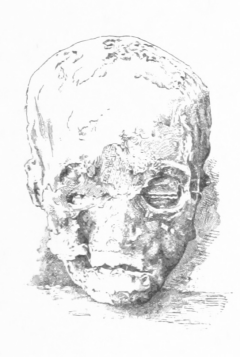
\includegraphics[scale=.5]{Skull}
  \end{center}


  \LEECHCRAFT[
    Name=Hair of the Dog,
    Link=leechcraft-hair-of-the-dog,
    Target=2,
    Keywords=Purge,
    Reversible=N
  ]

  Purge the effect of a Hang Over on a single person.

  \LEECHCRAFT[
    Name=Laudanum,
    Link=leechcraft-laudanum,
    Target=9,
    Keywords=Purge,
    Reversible=Y 
  ]

  Remove a Disgusted, Shaken, or Sickened effect on a single patient.  If applied during a Bivouac, Purge a single non-serious Mental Wound.   If desired, you can use this 'craft to cause a non-serious Mental wound (your choice) during a Bivouac.

  \LEECHCRAFT[
    Name=Mend,
    Link=leechcraft-mend,
    Target=2,
    Keywords=None,
    Reversible=Y
  ]

  Can only be applied to a patient who is Dying. Heal 1 Flesh.  

  You can also use Mend to cause a point of damage to a dying person (prompting a \DEATH roll).  The attempt isn't noticeable to others unless they're practiced in Leechcraft.

  \LEECHCRAFT[
    Name=Purge Toxin,
    Link=leechcraft-purge-toxin,
    Target=6,
    Keywords=None,
    Reversible=N 
  ]

  Immediately purge a Toxin from the body of a single patient

  \LEECHCRAFT[
    Name=Restore Senses,
    Link=leechcraft-restore-senses,
    Target=6,
    Keywords=None,
    Reversible=N 
  ]
  Remove a Blindness or Deafness effect on a single patient

  \LEECHCRAFT[
    Name=Sew Wounds,
    Link=leechcraft-sew-wounds,
    Target=4,
    Keywords=None,
    Reversible=N
  ]
  You can only perform this during a Breather or Bivouac. The patient rolls 1 \FLESH and heals that much Flesh.

  \LEECHCRAFT[
    Name=Smelling Salts,
    Link=leechcraft-smelling-salts,
    Target=3,
    Keywords=Purge,
    Reversible=N
  ]
  Purge a Knocked Out effect on a single patient


  \LEECHCRAFT[
    Name=Staunch,
    Link=leechcraft-staunch,
    Target=4,
    Keywords=Purge,
    Reversible=Y
  ]
  Purge or cause a Bleed effect on a single patient


  \LEECHCRAFT[
    Name=Trepanation,
    Link=leechcraft-trepanation,
    Target=8,
    Keywords=Purge,
    Reversible=Y  
  ]
  You can only drill holes in peoples' heads during a Bivouac.  Purge a Woozy effect on a single patient.   If desired, you can use this 'craft to cause the patient to become Woozy instead.

  \LEECHCRAFT[
    Name=Virtigo,
    Link=leechcraft-virtigo,
    Target=6,
    Keywords=None,
    Reversible=Y 
  ]
  
  Bivouac only.  Purge a Befuddled or Concussed effect on a single patient.   If desired, you can use this 'craft to cause the patient to become Befuddled or Concussed


